
\section{Introdução}




\noindent \begin{minipage}[c]{0.6\textwidth}
  \vspace {1cm}
  \begin{description}
    \item [CloudSim] De acordo com \citeonline{cloudSim}, é um framework para simulação de infraestrutura e serviços de computação em nuvem.
    É uma opção de aprendizado vastamente utilizado pelas universidades ao redor do globo, e uma framework de código aberto e qualquer um pode contribuir com a mesma através de seu repositório no \href{https://github.com/Cloudslab}{GitHub}.
    \item [Apache NetBeans]  O NetBeans é um software de desenvolvimento integrado (IDE), sobre distribuição da licença Apache, versão 2.0, o projeto conta com código aberto e recebe contribuição de qualquer desenvolvedor que se proponha a ajudar através do \href{https://github.com/apache/netbeans-website/blob/master/netbeans.apache.org/src/content/index.adoc}{GitHub}.
\newline
    \par Site do software: \href{https://netbeans.apache.org/}{Apache NetBeans}
  \end{description}

\end{minipage}
\begin{minipage}[c]{0.4\textwidth}

  
\includegraphics[width=\textwidth]{figure/netBeana.png}
  	\label{fig:netBeans}
    \captionof{figure}{NetBeans, \cite{netBeans}}
    %\captionof*{figure}{Fonte: \citeonline{linux:2023}}
\end{minipage}

\section{Métodos}
\par Para a elaboração da aula prática foi seguido o roteiro e um vídeo explicativo, disponibilizado pelos professores orientadores. Dentre orientações é definido uma sequência da passos para  confecão desta presente aula prática. No entanto, para este caso expecífico não foi necessário atualizar o pacote \href{https://www.oracle.com/java/technologies/downloads/}{Java JDK}, entre tudo, necessitei baixar o \href{https://netbeans.apache.org/download/nb19/}{NetBeans 18} e o \href{https://github.com/Cloudslab/cloudsim/releases}{CloudSim 2.1}, friso que o CloudSim possui versões novas (v6.0), no entanto, foi sugerido que usássemos a versão 2.1.

\par Para início da elaboração desta aula prática, foi prosseguido com a criação de um novo projeo na IDE NetBeans\ref{fig:netBeans}, conforme demonstrado nas figuras:\ref{fig:creat_project},\ref{fig:creat_project_name}

\begin{figure}[H]
    \center
    \subfigure[ Criação do projeto.\label{fig:creat_project}]{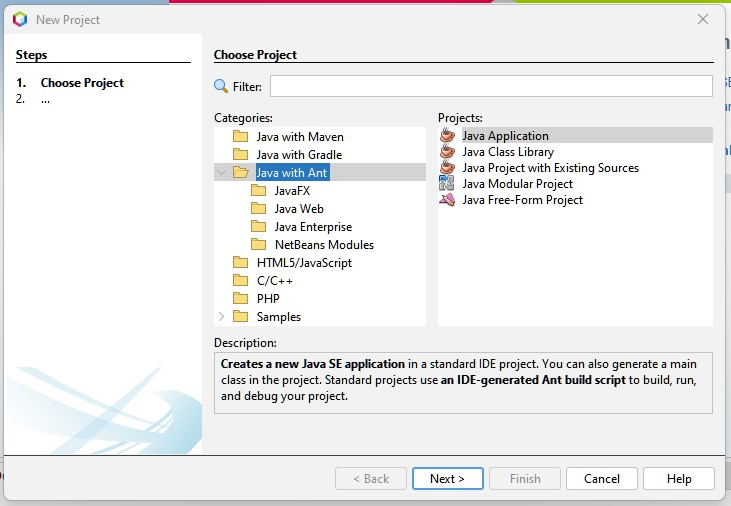
\includegraphics[scale=0.5]{figure/create_project.jpg}}
    \subfigure[Definição do nome do projeto.\label{fig:creat_project_name}]{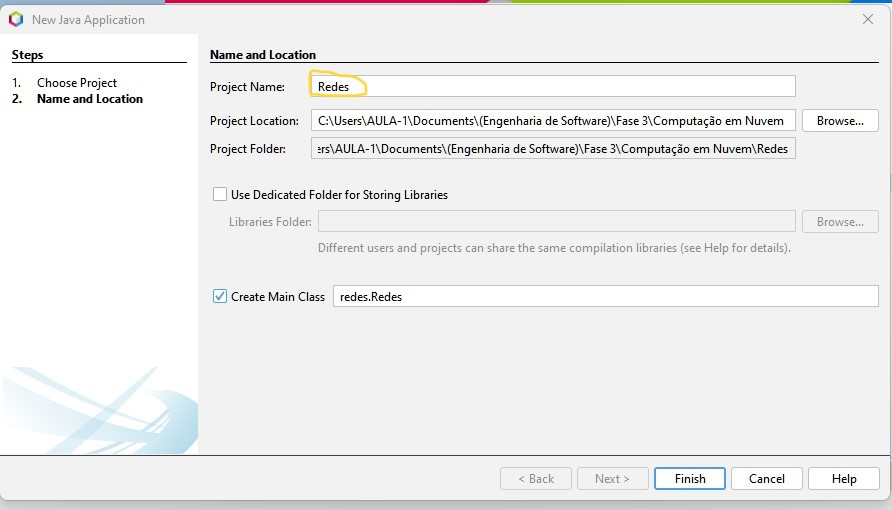
\includegraphics[scale=.5]{figure/create_project_name.jpg}}
    \caption{Etapas para a criação do projeto na IDE, O autor}\label{fig:confi_project}
\end{figure}
\par Como sugestão do roteiro o nome do projeto, foi definido como: \verb#Redes#, como demonstrado na Figura \ref{fig:creat_project_name}. De forma geral e para entendimento, este nome poderia ser qualquer outro desde que o fose alterado no projeto o nome da classe, conforme é demonstrado na figura \ref{fig:rename_pacote}, para o nome criado.



\section{Resultados}
\par De acordo com \citeonline{cloudSim:tutorial}, o que impulsiona o mecanismo de simulação central do CloudSim é o pacote que posui no dir: \verb#org.cloudbus.cloudsim.core#, com a explanação de uma fração do código vemos


\par Após a criação do projeto foi necessário alguns ajustes no projeto para que o exemplo \verb#CloudSimExample1.java# compilase na IDE, este ajustes podem ser explanados nas figuras abaixo.

\begin{enumerate}[label=\Roman{*}, ref=(\roman{*})]
  \item Foi necessário a alteração no nome do pacote, para \verb#Redes#, Conforme a figura \ref{fig:rename_pacote}. \newline
  \begin{figure}[h]
    \center
    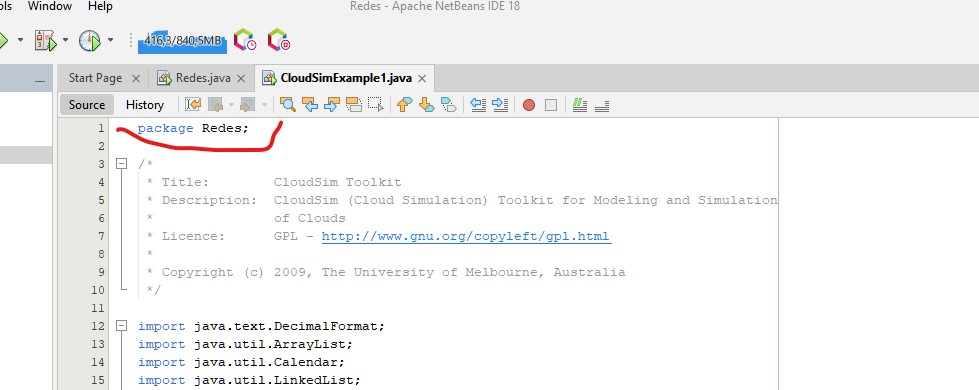
\includegraphics[scale=.5]{figure/rename_pacote.jpg}
    \caption{Alteração do nome do pacote, O autor}
    \label{fig:rename_pacote}
  \end{figure}

  \item Nessesario a inclusão do pacote \verb#jar# do CloudSim 2.1 que esta disponível nos documentos de downloads: \verb#\Computação em Nuvem\cloudsim-2.1\cloudsim-2.1\jars#, conforme a figura \ref{fig:import_jar}. \newline
  \begin{figure}[h]
    \center
    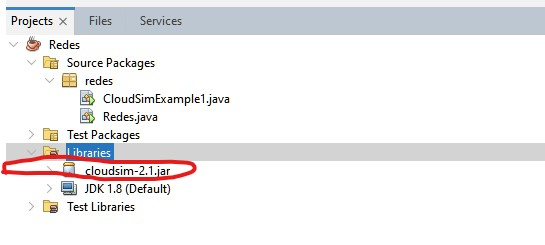
\includegraphics[scale=.8]{figure/import_jar.jpg}
    \caption{Importação do jar, O autor}
    \label{fig:import_jar}
  \end{figure}
\end{enumerate}
\newpage
\par Após os ajuste necessários, foi compilado o exemplo e o resultado da aula prática é observado na figura \ref{fig:result_pratic}.

\begin{figure}[h]
  \center
  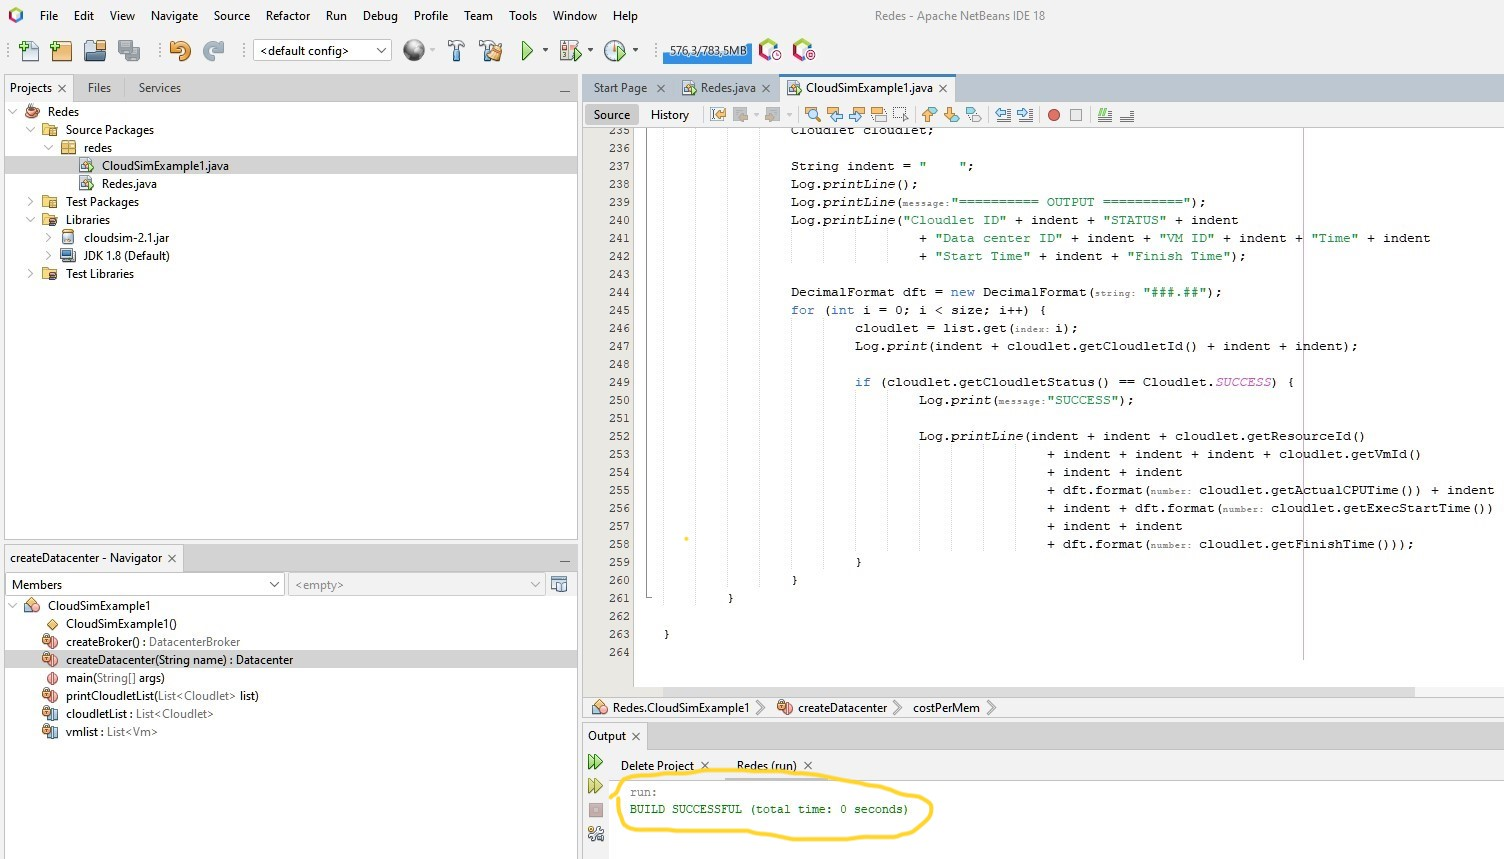
\includegraphics[width=\textwidth]{figure/result_pratic.jpg}
  \caption{Resultado da aula prática, O autor}
  \label{fig:result_pratic}
\end{figure}


\section{Conclusões}






  %$X \xLongleftarrow[\text{NATAN}]{\text{OGLIARI}} Y $ %COM TEXTO
	% $\uparrow$ %Seta para Cima
	%$\overleftarrow{NATAN}$
